\sep
\section{Grundlagen}
\Satz[1.1.2]  $\R$ ist ein kommutativer, angeordneter Körper, der ordnungsvollständig ist
\sep

\subsection{Infimum und Supremum}
\Def[1.1.12]  Sei $A \subset \R$ eine Teilmenge.
\begin{enumerate}
\item[1)]  $c \in \R$ ist \textbf{obere Schranke} if  $\forall a \in A: a \leqslant c$
\item[2)]  $c \in \R$ ist \textbf{untere Schranke} if $\forall a \in A: c \leqslant a$
\item[3)] $m \in \R$ heisst ein \textbf{Maximum} von A if $m \in A$ und $m$ eine obere Schranke von A ist.
\item[4)] $m \in \R$ heisst ein \textbf{Minimum} von A if $m \in A$ und $m$ eine untere Schranke von A ist.
\end{enumerate}

\Satz[1.1.15]. Sei $A \subset \R, A \neq \varnothing$ und beschränkt
\begin{enumerate}
\item[1)]  Kleinste obere Schranke: $\sup A$ (\textbf{Supremum})
\item[2)]  Grösste untere Schranke: $\inf A $ (\textbf{Infimum})
\end{enumerate}

Eigenschaften von Supremum und Infimum
\begin{enumerate}
\item[•]  $\sup (A \cup B) = \text{max} (\sup A, \sup B)$
\item[•]  $\sup (A + B) = \sup A + \sup B$
\item[•]  $\inf (A \cup B) = \text{min} (\inf A, \inf B)$
\item[•]  $\inf (A + B) = \inf A + \inf B$
\end{enumerate}

\sep

\subsection{Random, but useful stuff}
Some middle school stuff that might come in handy

\sep

\subsubsection{Unit Circle $(\sin(x), \cos(x))$}
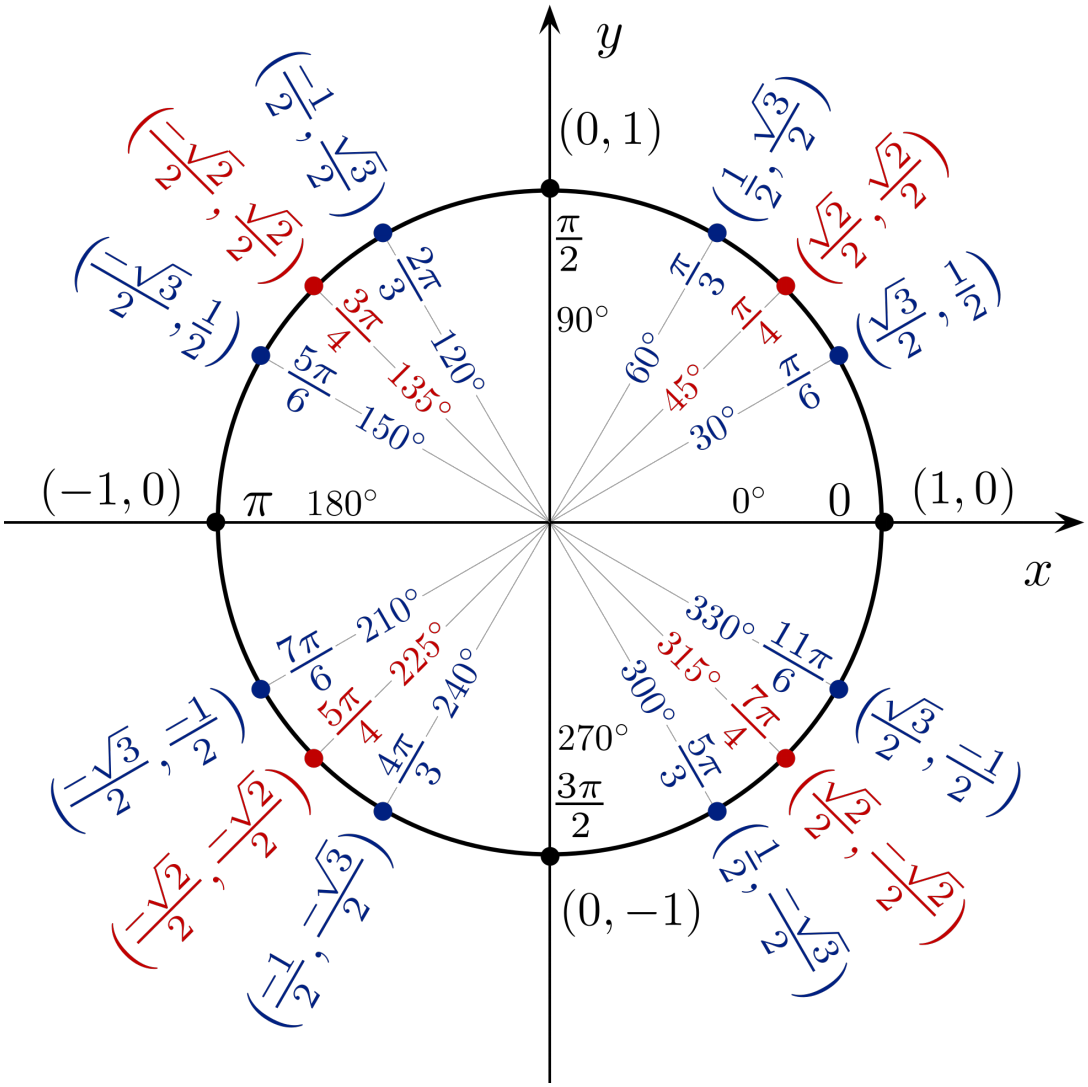
\includegraphics[scale=0.225]{sinus_cosinus}

\sep

\subsubsection{Quadratic Formula for $a x^2 + b x + c = 0$}

\[ x = \frac{-b + \pm \sqrt{b^2 - 4 a c} }{2 a} \]